\subsection{Eksempel på problem med udvidelser} \label{kap:grafen_for_udvidet}
Vi kan nu på samme måde som med basisproblemet opstille et simplificeret eksempel på det udvidede problem for på den måde at illustrere, hvordan man finder den mest profitable vej igennem en graf af denne problemtype. Vi opstiller en orienteret, simpel, vægtet graf, hvor vi benytter følgende data:

\begin{itemize}
  \item $t \in \{1,2,3,4,5,6\}$
  \item $q_{0}=1$
  \item $q_{\min \_ \textrm{liste}}=[0,1,1,0,0,0]$
  \item $q_{\max \_ \textrm{liste}}=[2,3,3,2,2,2]$
  \item $i_{\max \_ \textrm{liste}}=[1,2,1,2,1,1]$
  \item $u_{\max \_ \textrm{liste}}=[1,2,1,2,1,1]$
  \item $p_{t}=(20,22,25,18,15,15)$
  \item $q_{\goal}=0$
  \item $\kappa=0,7$
\end{itemize}

I eksemplet tager vi igen kun udgangspunkt i seks måneder. Denne gang ændrer grænserne for antallet af gasenheder, der må sælges og købes, sig løbende i de forskellige måneder. På samme måde ændrer grænserne for lagerbeholdningen sig. Vi opstiller følgende graf med de givne vægte:

\begin{figure}[H]
\centering
	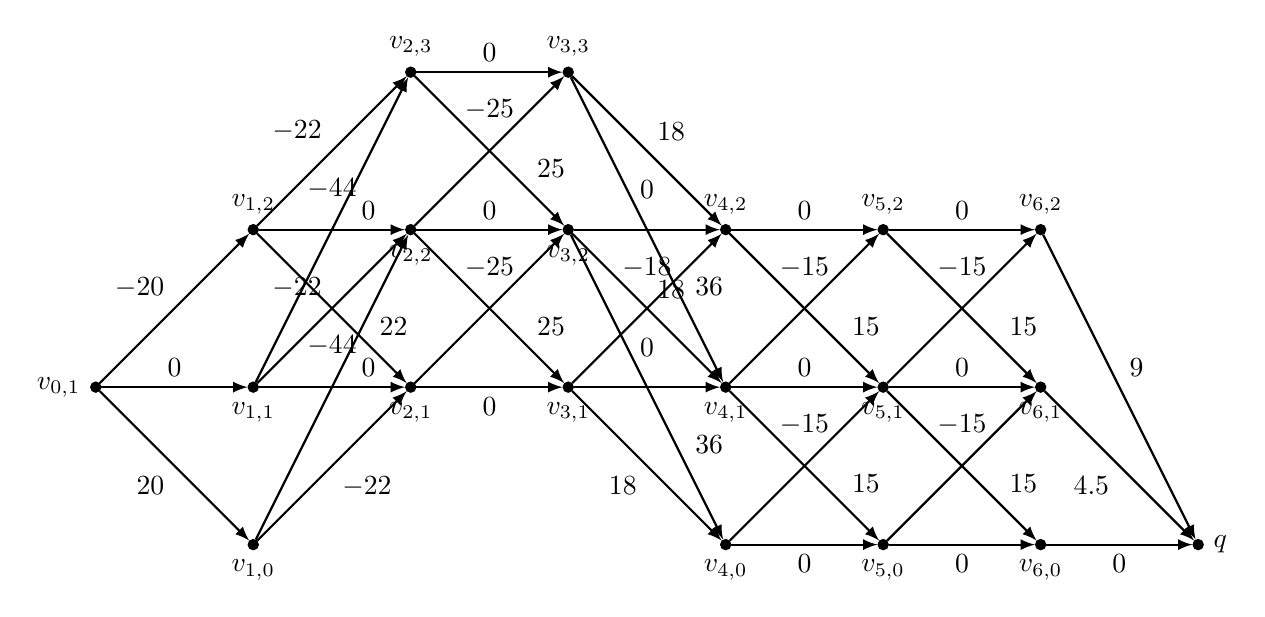
\begin{tikzpicture}

       \tikzset{enclosed/.style={draw, circle, inner sep=0pt, minimum size=.13cm, fill=black}}
%% Vertices
      	\node[enclosed, label={left:  $v_{0,1}$}]   (v1) at  (0,2)  {};
      	\node[enclosed, label={below: $v_{1,0}$}]   (v2) at  (2,0)  {};
    	\node[enclosed, label={below: $v_{1,1}$}]   (v3) at  (2,2)  {};
  	    \node[enclosed, label={above: $v_{1,2}$}]   (v4) at  (2,4)  {};
     	\node[enclosed, label={below: $v_{2,1}$}]   (v5) at  (4,2)  {};
     	\node[enclosed, label={below: $v_{2,2}$}]   (v6) at  (4,4)  {};
     	\node[enclosed, label={above: $v_{2,3}$}]   (v7) at  (4,6)  {};
     	\node[enclosed, label={below: $v_{3,1}$}]   (v8) at  (6,2)  {};
     	\node[enclosed, label={below: $v_{3,2}$}]   (v9) at  (6,4)  {};
     	\node[enclosed, label={above: $v_{3,3}$}]   (v10) at (6,6)  {};
     	\node[enclosed, label={below: $v_{4,0}$}]   (v11) at (8,0)  {};
     	\node[enclosed, label={below: $v_{4,1}$}]   (v12) at (8,2)  {};
      	\node[enclosed, label={above: $v_{4,2}$}]   (v13) at (8,4)  {};
  	    \node[enclosed, label={below: $v_{5,0}$}]   (v14) at (10,0) {};
  	    \node[enclosed, label={below: $v_{5,1}$}]   (v15) at (10,2) {};
     	\node[enclosed, label={above: $v_{5,2}$}]   (v16) at (10,4) {};
     	\node[enclosed, label={below: $v_{6,0}$}]   (v17) at (12,0) {};
     	\node[enclosed, label={below: $v_{6,1}$}]   (v18) at (12,2) {};
     	\node[enclosed, label={above: $v_{6,2}$}]   (v19) at (12,4) {};
     	\node[enclosed, label={right: $q_{\slut}$}] (v20) at (14,0) {};
   
%Edges
		\path[->,>=latex,thick] (v1) edge node[midway, sloped, above, label={below, black: $20$}] {} (v2);
		\path[->,>=latex,thick] (v1) edge node[midway, sloped, below, label={above: $0$ }] {} (v3);
		\path[->,>=latex,thick] (v1) edge node[midway, sloped, below, label={above, black: $-20$ }] {} (v4);
		\path[->,>=latex,thick] (v2) edge node[midway, sloped, above, label={below: $-22$ }] {} (v5);
		\path[->,>=latex,thick] (v2) edge node[midway, above, label={above: $-44$ }] {} (v6);
		\path[->,>=latex,thick] (v3) edge node[near end, sloped, below, label={above: $0$ }] {} (v5);
		\path[->,>=latex,thick] (v3) edge node[midway, sloped, below, label={above: $-22$ }] {} (v6);
		\path[->,>=latex,thick] (v3) edge node[midway, above, label={above: $-44$ }] {} (v7);
		\path[->,>=latex,thick] (v4) edge node[near end, sloped, below, label={above, black: $22$ }] {} (v5);
		\path[->,>=latex,thick] (v4) edge node[near end, sloped, below, label={above, black: $0$ }] {} (v6);		
		\path[->,>=latex,thick] (v4) edge node[midway, sloped, below, label={above: $-22$ }] {} (v7);
		\path[->,>=latex,thick] (v5) edge node[midway, sloped, above, label={below: $0$ }] {} (v8);
		\path[->,>=latex,thick] (v5) edge node[midway, above, label={above: $-25$ }] {} (v9);
		\path[->,>=latex,thick] (v6) edge node[near end, sloped, below, label={above,black: $25$ }] {} (v8);
		\path[->,>=latex,thick] (v6) edge node[midway, sloped, below, label={above: $0$ }] {} (v9);
		\path[->,>=latex,thick] (v6) edge node[midway, above, label={above: $-25$ }] {} (v10);
		\path[->,>=latex,thick] (v7) edge node[near end, sloped, below, label={above: $25$ }] {} (v9);
		\path[->,>=latex,thick] (v7) edge node[midway, sloped, below, label={above: $0$ }] {} (v10);
		\path[->,>=latex,thick] (v8) edge node[midway, sloped, above, label={below,black: $18$ }] {} (v11);
		\path[->,>=latex,thick] (v8) edge node[midway, above, label={above: $0$ }] {} (v12);
		\path[->,>=latex,thick] (v8) edge node[midway, above, label={above: $-18$ }] {} (v13);
		\path[->,>=latex,thick] (v9) edge node[near end, sloped, below, label={above: $36$ }] {} (v11);
		\path[->,>=latex,thick] (v9) edge node[midway, sloped, below, label={above: $18$ }] {} (v12);
		\path[->,>=latex,thick] (v9) edge node[midway, above, label={above: $0$ }] {} (v13);
		\path[->,>=latex,thick] (v10) edge node[near end, sloped, below, label={above: $36$ }] {} (v12);
		\path[->,>=latex,thick] (v10) edge node[midway, sloped, below, label={above: $18$ }] {} (v13);
		\path[->,>=latex,thick] (v11) edge node[midway, sloped, above, label={below,black: $0$ }] {} (v14);
		\path[->,>=latex,thick] (v11) edge node[midway, above, label={above,black: $-15$ }] {} (v15);
		\path[->,>=latex,thick] (v12) edge node[near end, sloped, below, label={above: $15$ }] {} (v14);
		\path[->,>=latex,thick] (v12) edge node[midway, sloped, below, label={above: $0$ }] {} (v15);
		\path[->,>=latex,thick] (v12) edge node[midway, above, label={above: $-15$ }] {} (v16);
		\path[->,>=latex,thick] (v13) edge node[near end, sloped, below, label={above: $15$ }] {} (v15);
		\path[->,>=latex,thick] (v13) edge node[midway, sloped, below, label={above: $0$ }] {} (v16);
		\path[->,>=latex,thick] (v14) edge node[midway, sloped, above, label={below,black: $0$ }] {} (v17);
		\path[->,>=latex,thick] (v14) edge node[midway, above, label={above,black: $-15$ }] {} (v18);
		\path[->,>=latex,thick] (v15) edge node[near end, sloped, below, label={above: $15$ }] {} (v17);
		\path[->,>=latex,thick] (v15) edge node[midway, sloped, below, label={above: $0$ }] {} (v18);
		\path[->,>=latex,thick] (v15) edge node[midway, above, label={above,black: $-15$ }] {} (v19);
		\path[->,>=latex,thick] (v16) edge node[near end, sloped, below, label={above: $15$ }] {} (v18);
		\path[->,>=latex,thick] (v16) edge node[midway, sloped, below, label={above: $0$ }] {} (v19);
		\path[->,>=latex,thick] (v17) edge node[midway, sloped, above, label={below,black: $0$ }] {} (v20);
		\path[->,>=latex,thick] (v18) edge node[midway, sloped, above, label={below,black: $4.5$ }] {} (v20);
		\path[->,>=latex,thick] (v19) edge node[midway, sloped, below, label={above,black: $9$ }] {} (v20);
	\end{tikzpicture}
	\caption{Forsimplet graf for udvidet problem.}
	\label{fig.gaslager_udvidet}
\end{figure}

Vi ønsker igen at maksimere overskuddet og dermed finde den længste vej fra $v_{0,1}$ til $q_{\slut}$. For at løse problemet som et korteste vej-problem ganger vi igen med -1 og får dermed den omvendte graf:

\begin{figure}[H]
\centering
	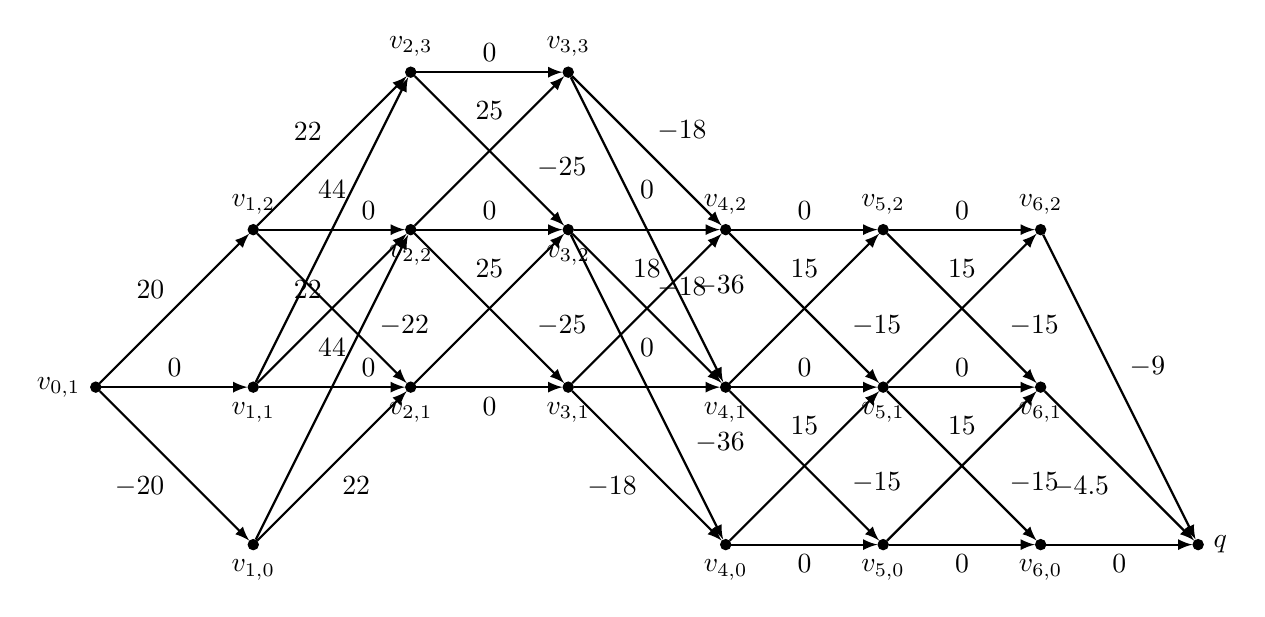
\begin{tikzpicture}

       \tikzset{enclosed/.style={draw, circle, inner sep=0pt, minimum size=.13cm, fill=black}}
%% Vertices
      	\node[enclosed, label={left:  $v_{0,1}$}]   (v1) at  (0,2)  {};
      	\node[enclosed, label={below: $v_{1,0}$}]   (v2) at  (2,0)  {};
    	\node[enclosed, label={below: $v_{1,1}$}]   (v3) at  (2,2)  {};
  	    \node[enclosed, label={above: $v_{1,2}$}]   (v4) at  (2,4)  {};
     	\node[enclosed, label={below: $v_{2,1}$}]   (v5) at  (4,2)  {};
     	\node[enclosed, label={below: $v_{2,2}$}]   (v6) at  (4,4)  {};
     	\node[enclosed, label={above: $v_{2,3}$}]   (v7) at  (4,6)  {};
     	\node[enclosed, label={below: $v_{3,1}$}]   (v8) at  (6,2)  {};
     	\node[enclosed, label={below: $v_{3,2}$}]   (v9) at  (6,4)  {};
     	\node[enclosed, label={above: $v_{3,3}$}]   (v10) at (6,6)  {};
     	\node[enclosed, label={below: $v_{4,0}$}]   (v11) at (8,0)  {};
     	\node[enclosed, label={below: $v_{4,1}$}]   (v12) at (8,2)  {};
      	\node[enclosed, label={above: $v_{4,2}$}]   (v13) at (8,4)  {};
  	    \node[enclosed, label={below: $v_{5,0}$}]   (v14) at (10,0) {};
  	    \node[enclosed, label={below: $v_{5,1}$}]   (v15) at (10,2) {};
     	\node[enclosed, label={above: $v_{5,2}$}]   (v16) at (10,4) {};
     	\node[enclosed, label={below: $v_{6,0}$}]   (v17) at (12,0) {};
     	\node[enclosed, label={below: $v_{6,1}$}]   (v18) at (12,2) {};
     	\node[enclosed, label={above: $v_{6,2}$}]   (v19) at (12,4) {};
     	\node[enclosed, label={right: $q_{\slut}$}] (v20) at (14,0) {};
     	
%Edges
		\path[->,>=latex,thick] (v1) edge node[midway, sloped, above, label={below, black: $-20$}] {} (v2);
		\path[->,>=latex,thick] (v1) edge node[midway, sloped, below, label={above: $0$ }] {} (v3);
		\path[->,>=latex,thick] (v1) edge node[midway, sloped, below, label={above, black: $20$ }] {} (v4);
		\path[->,>=latex,thick] (v2) edge node[midway, sloped, above, label={below: $22$ }] {} (v5);
		\path[->,>=latex,thick] (v2) edge node[midway, above, label={above: $44$ }] {} (v6);
		\path[->,>=latex,thick] (v3) edge node[near end, sloped, below, label={above: $0$ }] {} (v5);
		\path[->,>=latex,thick] (v3) edge node[midway, sloped, below, label={above: $22$ }] {} (v6);
		\path[->,>=latex,thick] (v3) edge node[midway, above, label={above: $44$ }] {} (v7);
		\path[->,>=latex,thick] (v4) edge node[near end, sloped, below, label={above, black: $-22$ }] {} (v5);
		\path[->,>=latex,thick] (v4) edge node[near end, sloped, below, label={above, black: $0$ }] {} (v6);		
		\path[->,>=latex,thick] (v4) edge node[midway, sloped, below, label={above: $22$ }] {} (v7);
		\path[->,>=latex,thick] (v5) edge node[midway, sloped, above, label={below: $0$ }] {} (v8);
		\path[->,>=latex,thick] (v5) edge node[midway, above, label={above: $25$ }] {} (v9);
		\path[->,>=latex,thick] (v6) edge node[near end, sloped, below, label={above,black: $-25$ }] {} (v8);
		\path[->,>=latex,thick] (v6) edge node[midway, sloped, below, label={above: $0$ }] {} (v9);
		\path[->,>=latex,thick] (v6) edge node[midway, above, label={above: $25$ }] {} (v10);
		\path[->,>=latex,thick] (v7) edge node[near end, sloped, below, label={above: $-25$ }] {} (v9);
		\path[->,>=latex,thick] (v7) edge node[midway, sloped, below, label={above: $0$ }] {} (v10);
		\path[->,>=latex,thick] (v8) edge node[midway, sloped, above, label={below,black: $-18$ }] {} (v11);
		\path[->,>=latex,thick] (v8) edge node[midway, above, label={above: $0$ }] {} (v12);
		\path[->,>=latex,thick] (v8) edge node[midway, above, label={above: $18$ }] {} (v13);
		\path[->,>=latex,thick] (v9) edge node[near end, sloped, below, label={above: $-36$ }] {} (v11);
		\path[->,>=latex,thick] (v9) edge node[midway, sloped, below, label={above: $-18$ }] {} (v12);
		\path[->,>=latex,thick] (v9) edge node[midway, above, label={above: $0$ }] {} (v13);
		\path[->,>=latex,thick] (v10) edge node[near end, sloped, below, label={above: $-36$ }] {} (v12);
		\path[->,>=latex,thick] (v10) edge node[midway, sloped, below, label={above: $-18$ }] {} (v13);
		\path[->,>=latex,thick] (v11) edge node[midway, sloped, above, label={below,black: $0$ }] {} (v14);
		\path[->,>=latex,thick] (v11) edge node[midway, above, label={above,black: $15$ }] {} (v15);
		\path[->,>=latex,thick] (v12) edge node[near end, sloped, below, label={above: $-15$ }] {} (v14);
		\path[->,>=latex,thick] (v12) edge node[midway, sloped, below, label={above: $0$ }] {} (v15);
		\path[->,>=latex,thick] (v12) edge node[midway, above, label={above: $15$ }] {} (v16);
		\path[->,>=latex,thick] (v13) edge node[near end, sloped, below, label={above: $-15$ }] {} (v15);
		\path[->,>=latex,thick] (v13) edge node[midway, sloped, below, label={above: $0$ }] {} (v16);
		\path[->,>=latex,thick] (v14) edge node[midway, sloped, above, label={below,black: $0$ }] {} (v17);
		\path[->,>=latex,thick] (v14) edge node[midway, above, label={above,black: $15$ }] {} (v18);
		\path[->,>=latex,thick] (v15) edge node[near end, sloped, below, label={above: $-15$ }] {} (v17);
		\path[->,>=latex,thick] (v15) edge node[midway, sloped, below, label={above: $0$ }] {} (v18);
		\path[->,>=latex,thick] (v15) edge node[midway, above, label={above,black: $15$ }] {} (v19);
		\path[->,>=latex,thick] (v16) edge node[near end, sloped, below, label={above: $-15$ }] {} (v18);
		\path[->,>=latex,thick] (v16) edge node[midway, sloped, below, label={above: $0$ }] {} (v19);
		\path[->,>=latex,thick] (v17) edge node[midway, sloped, above, label={below,black: $0$ }] {} (v20);
		\path[->,>=latex,thick] (v18) edge node[midway, sloped, above, label={below,black: $-4.5$ }] {} (v20);
		\path[->,>=latex,thick] (v19) edge node[midway, sloped, below, label={above,black: $-9$ }] {} (v20);
	\end{tikzpicture}
	\caption{Forsimplet, omvendt graf for udvidet problem.}
	\label{fig.omvendt_udvidet}
\end{figure}

Vi kan nu løse problemet som et korteste vej-problem ved igen at bruge Dijkstras algoritme. Derfor lægger vi nu 40 til alle tal i grafen, så der ikke optræder negative kantvægte. Vi får nu den omvendte graf med udelukkende ikke-negative værdier:


\begin{figure}[H]
\centering
	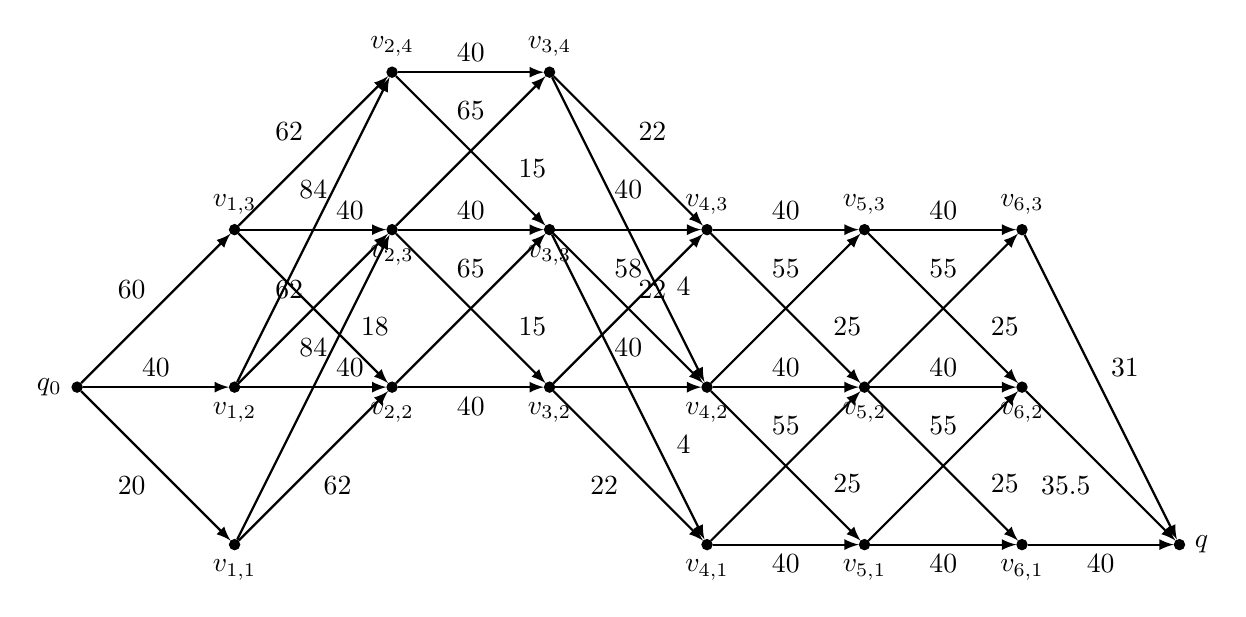
\begin{tikzpicture}

       \tikzset{enclosed/.style={draw, circle, inner sep=0pt, minimum size=.13cm, fill=black}}
%% Vertices
      	\node[enclosed, label={left:  $q_{0}$}]     (v1) at  (0,2)  {};
      	\node[enclosed, label={below: $v_{1,1}$}]   (v2) at  (2,0)  {};
    		\node[enclosed, label={below: $v_{1,2}$}]   (v3) at  (2,2)  {};
  	    \node[enclosed, label={above: $v_{1,3}$}]   (v4) at  (2,4)  {};
     	\node[enclosed, label={below: $v_{2,2}$}]   (v5) at  (4,2)  {};
     	\node[enclosed, label={below: $v_{2,3}$}]   (v6) at  (4,4)  {};
     	\node[enclosed, label={above: $v_{2,4}$}]   (v7) at  (4,6)  {};
     	\node[enclosed, label={below: $v_{3,2}$}]   (v8) at  (6,2)  {};
     	\node[enclosed, label={below: $v_{3,3}$}]   (v9) at  (6,4)  {};
     	\node[enclosed, label={above: $v_{3,4}$}]   (v10) at (6,6)  {};
     	\node[enclosed, label={below: $v_{4,1}$}]   (v11) at (8,0)  {};
     	\node[enclosed, label={below: $v_{4,2}$}]   (v12) at (8,2)  {};
      	\node[enclosed, label={above: $v_{4,3}$}]   (v13) at (8,4)  {};
  	    \node[enclosed, label={below: $v_{5,1}$}]   (v14) at (10,0) {};
  	    \node[enclosed, label={below: $v_{5,2}$}]   (v15) at (10,2) {};
     	\node[enclosed, label={above: $v_{5,3}$}]   (v16) at (10,4) {};
     	\node[enclosed, label={below: $v_{6,1}$}]   (v17) at (12,0) {};
     	\node[enclosed, label={below: $v_{6,2}$}]   (v18) at (12,2) {};
     	\node[enclosed, label={above: $v_{6,3}$}]   (v19) at (12,4) {};
     	\node[enclosed, label={right: $q_{\slut}$}] (v20) at (14,0) {};
     	
%Edges
		\path[->,>=latex,thick] (v1) edge node[midway, sloped, above, label={below, black: $20$}] {} (v2);
		\path[->,>=latex,thick] (v1) edge node[midway, sloped, below, label={above: $40$ }] {} (v3);
		\path[->,>=latex,thick] (v1) edge node[midway, sloped, below, label={above, black: $60$ }] {} (v4);
		\path[->,>=latex,thick] (v2) edge node[midway, sloped, above, label={below: $62$ }] {} (v5);
		\path[->,>=latex,thick] (v2) edge node[midway, above, label={above: $84$ }] {} (v6);
		\path[->,>=latex,thick] (v3) edge node[near end, sloped, below, label={above: $40$ }] {} (v5);
		\path[->,>=latex,thick] (v3) edge node[midway, sloped, below, label={above: $62$ }] {} (v6);
		\path[->,>=latex,thick] (v3) edge node[midway, above, label={above: $84$ }] {} (v7);
		\path[->,>=latex,thick] (v4) edge node[near end, sloped, below, label={above, black: $18$ }] {} (v5);
		\path[->,>=latex,thick] (v4) edge node[near end, sloped, below, label={above, black: $40$ }] {} (v6);		
		\path[->,>=latex,thick] (v4) edge node[midway, sloped, below, label={above: $62$ }] {} (v7);
		\path[->,>=latex,thick] (v5) edge node[midway, sloped, above, label={below: $40$ }] {} (v8);
		\path[->,>=latex,thick] (v5) edge node[midway, above, label={above: $65$ }] {} (v9);
		\path[->,>=latex,thick] (v6) edge node[near end, sloped, below, label={above,black: $15$ }] {} (v8);
		\path[->,>=latex,thick] (v6) edge node[midway, sloped, below, label={above: $40$ }] {} (v9);
		\path[->,>=latex,thick] (v6) edge node[midway, above, label={above: $65$ }] {} (v10);
		\path[->,>=latex,thick] (v7) edge node[near end, sloped, below, label={above: $15$ }] {} (v9);
		\path[->,>=latex,thick] (v7) edge node[midway, sloped, below, label={above: $40$ }] {} (v10);
		\path[->,>=latex,thick] (v8) edge node[midway, sloped, above, label={below,black: $22$ }] {} (v11);
		\path[->,>=latex,thick] (v8) edge node[midway, above, label={above: $40$ }] {} (v12);
		\path[->,>=latex,thick] (v8) edge node[midway, above, label={above: $58$ }] {} (v13);
		\path[->,>=latex,thick] (v9) edge node[near end, sloped, below, label={above: $4$ }] {} (v11);
		\path[->,>=latex,thick] (v9) edge node[midway, sloped, below, label={above: $22$ }] {} (v12);
		\path[->,>=latex,thick] (v9) edge node[midway, above, label={above: $40$ }] {} (v13);
		\path[->,>=latex,thick] (v10) edge node[near end, sloped, below, label={above: $4$ }] {} (v12);
		\path[->,>=latex,thick] (v10) edge node[midway, sloped, below, label={above: $22$ }] {} (v13);
		\path[->,>=latex,thick] (v11) edge node[midway, sloped, above, label={below,black: $40$ }] {} (v14);
		\path[->,>=latex,thick] (v11) edge node[midway, above, label={above,black: $55$ }] {} (v15);
		\path[->,>=latex,thick] (v12) edge node[near end, sloped, below, label={above: $25$ }] {} (v14);
		\path[->,>=latex,thick] (v12) edge node[midway, sloped, below, label={above: $40$ }] {} (v15);
		\path[->,>=latex,thick] (v12) edge node[midway, above, label={above: $55$ }] {} (v16);
		\path[->,>=latex,thick] (v13) edge node[near end, sloped, below, label={above: $25$ }] {} (v15);
		\path[->,>=latex,thick] (v13) edge node[midway, sloped, below, label={above: $40$ }] {} (v16);
		\path[->,>=latex,thick] (v14) edge node[midway, sloped, above, label={below,black: $40$ }] {} (v17);
		\path[->,>=latex,thick] (v14) edge node[midway, above, label={above,black: $55$ }] {} (v18);
		\path[->,>=latex,thick] (v15) edge node[near end, sloped, below, label={above: $25$ }] {} (v17);
		\path[->,>=latex,thick] (v15) edge node[midway, sloped, below, label={above: $40$ }] {} (v18);
		\path[->,>=latex,thick] (v15) edge node[midway, above, label={above,black: $55$ }] {} (v19);
		\path[->,>=latex,thick] (v16) edge node[near end, sloped, below, label={above: $25$ }] {} (v18);
		\path[->,>=latex,thick] (v16) edge node[midway, sloped, below, label={above: $40$ }] {} (v19);
		\path[->,>=latex,thick] (v17) edge node[midway, sloped, above, label={below,black: $40$ }] {} (v20);
		\path[->,>=latex,thick] (v18) edge node[midway, sloped, above, label={below,black: $35.5$ }] {} (v20);
		\path[->,>=latex,thick] (v19) edge node[midway, sloped, below, label={above,black: $31$ }] {} (v20);
	\end{tikzpicture}
	\caption{Omvendt, positiv, udvidet graf.}
	\label{fig.omvendt_udvidet}
\end{figure}

Vi kan på samme måde som ved basisproblemet opstille en tabel over de mulige veje gennem grafen fra $v_{0,1}$ til $q_{\slut}$:

\begin{table}[H]
\centering
\begin{tabular}{|c|c|c|c|c|c|c|c|c|c|c|c|c|c|} 
\hline
$n$ & $R_{n} \bigcup$ & $q_{0}$ & $v_{1,1}$ & $v_{1,2}$ & $v_{1,3}$ & $v_{2,2}$ & $v_{2,3}$ & $v_{2,4}$ & $\ldots$ & $v_{6,1}$ & $v_{6,2}$ & $v_{6,3}$ & $q_{slut}$ \\
\hline
0 & $\emptyset$ & 0 & $\infty$ & $\infty$ & $\infty$ & $\infty$ & $\infty$ & $\infty$ & $\ldots$ & $\infty$ & $\infty$ & $\infty$ & $\infty$ \\ 
1 & $q_{0}$ & & 20 & 40 & 60 & $\infty$ & $\infty$ & $\infty$ & $\ldots$ & $\infty$ & $\infty$ & $\infty$ & $\infty$\\ 
2 & $v_{1,1}$ & & & 40 & 60 & 82 & 104 & $\infty$ & $\ldots$ & $\infty$ & $\infty$ & $\infty$ & $\infty$\\ 
3 & $v_{1,2}$ & & & & 60 & 80 & 102 & 124 & $\ldots$ & $\infty$ & $\infty$ & $\infty$ & $\infty$\\
4 & $v_{1,3}$ & & & & & 78 & 100 & 122 & $\ldots$ & $\infty$ & $\infty$ & $\infty$ & $\infty$\\ 
5 & $v_{2,2}$ & & & & & & 100 & 122 & $\ldots$ & $\infty$ & $\infty$ & $\infty$ & $\infty$\\ 
6 & $v_{2,3}$ & & & & & & & 122 & $\ldots$ & $\infty$ & $\infty$ & $\infty$ & $\infty$\\  
$\vdots$ & $\vdots$ & $\vdots$ & $\vdots$ & $\vdots$ & $\vdots$ & $\vdots$ & $\vdots$ & $\vdots$ &  & $\vdots$ & $\vdots$ & $\vdots$ & $\vdots$\\ 
14 & $v_{5,1}$ &  &  &  &  &  &  &  & $\ldots$ & 217 & 232 & $\infty$ & $\infty$\\ 
15 & $v_{5,2}$ &  &  &  &  &  &  &  & $\ldots$ & 217 & 232 & 247 & $\infty$\\ 
16 & $v_{5,3}$ &  &  &  &  &  &  &  & $\ldots$ & 217 & 232 & 247 & $\infty$\\ 
17 & $v_{6,1}$ &  &  &  &  &  &  &  & $\ldots$ &  & 232 & 247 & 257\\ 
18 & $v_{6,2}$ &  &  &  &  &  &  &  & $\ldots$ &  &  & 247 & 257\\ 
18 & $v_{6,3}$ &  &  &  &  &  &  &  & $\ldots$ &  &  &  & 257\\ 
\hline
\end{tabular}
\caption{Tabel over veje gennem forsimplet, udvidet graf.}
\label{table:forsimplet_udvidet_graf}
\end{table} 


Beregningerne foregår på samme vis som i \autoref{table:forsimplet_graf}. Vi får dermed, at vi har to forskellige veje fra $v_{0,1}$ til $q_{\slut}$, som begge har distancen 257. I den oprindelige graf i \autoref{fig.gaslager_udvidet} havde kanterne andre vægte, som vi nu kan indsætte igen efter brugen af Dijkstras algoritme. Vejen går igennem de samme knuder, og ønsker vi at finde distancen fra $v_{0,1}$ til $q_{\slut}$, skal vi blot tage vores resultat og trække de 40, som vi adderede hver kant med, fra 7 gange, altså en gang for hver kant i vejen fra $v_{0,1}$ til $q_{\slut}$. Derefter ganger vi med -1.
\begin{equation}
(257-40 \cdot 7)(-1) = 23.
\end{equation}
Vejene illustreres på \autoref{fig:gaslager_udvidet}:

\begin{figure}[H]
\centering
	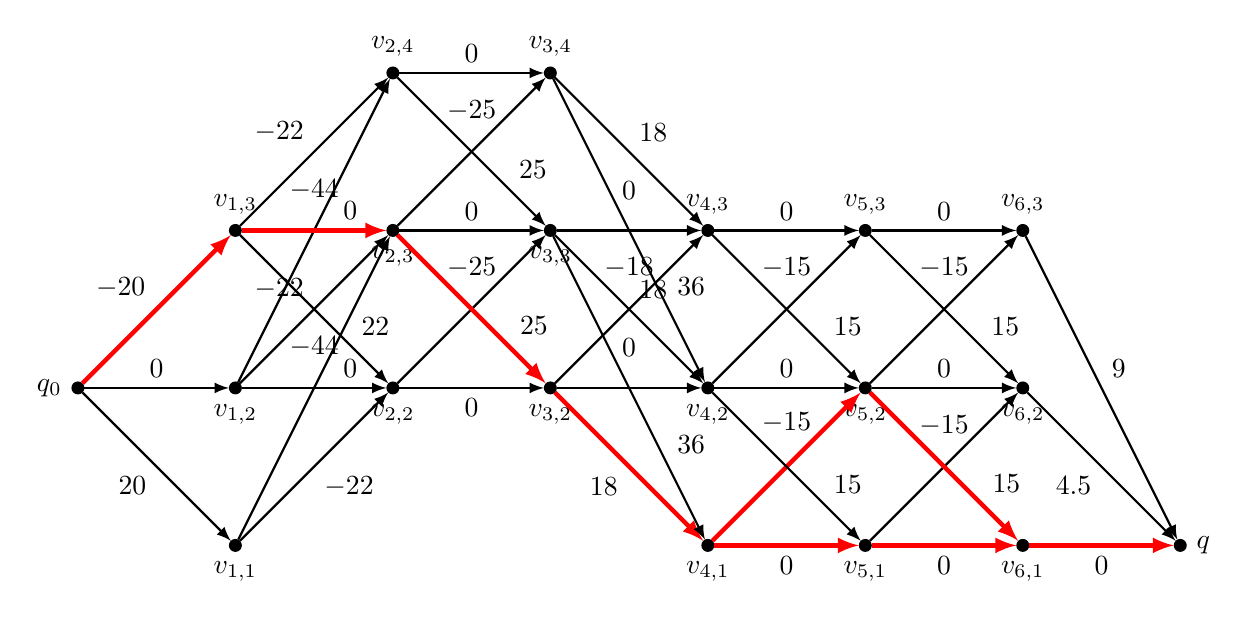
\begin{tikzpicture}

       \tikzset{enclosed/.style={draw, circle, inner sep=0pt, minimum size=.15cm, fill=black}}
%% Vertices
      	\node[enclosed, label={left:  $q_{0}$}]     (v1) at  (0,2)  {};
      	\node[enclosed, label={below: $v_{1,1}$}]   (v2) at  (2,0)  {};
    		\node[enclosed, label={below: $v_{1,2}$}]   (v3) at  (2,2)  {};
  	    \node[enclosed, label={above: $v_{1,3}$}]   (v4) at  (2,4)  {};
     	\node[enclosed, label={below: $v_{2,2}$}]   (v5) at  (4,2)  {};
     	\node[enclosed, label={below: $v_{2,3}$}]   (v6) at  (4,4)  {};
     	\node[enclosed, label={above: $v_{2,4}$}]   (v7) at  (4,6)  {};
     	\node[enclosed, label={below: $v_{3,2}$}]   (v8) at  (6,2)  {};
     	\node[enclosed, label={below: $v_{3,3}$}]   (v9) at  (6,4)  {};
     	\node[enclosed, label={above: $v_{3,4}$}]   (v10) at (6,6)  {};
     	\node[enclosed, label={below: $v_{4,1}$}]   (v11) at (8,0)  {};
     	\node[enclosed, label={below: $v_{4,2}$}]   (v12) at (8,2)  {};
      	\node[enclosed, label={above: $v_{4,3}$}]   (v13) at (8,4)  {};
  	    \node[enclosed, label={below: $v_{5,1}$}]   (v14) at (10,0) {};
  	    \node[enclosed, label={below: $v_{5,2}$}]   (v15) at (10,2) {};
     	\node[enclosed, label={above: $v_{5,3}$}]   (v16) at (10,4) {};
     	\node[enclosed, label={below: $v_{6,1}$}]   (v17) at (12,0) {};
     	\node[enclosed, label={below: $v_{6,2}$}]   (v18) at (12,2) {};
     	\node[enclosed, label={above: $v_{6,3}$}]   (v19) at (12,4) {};
     	\node[enclosed, label={right: $q_{\slut}$}] (v20) at (14,0) {};
     	
%Edges
		\path[->,>=latex,thick] (v1) edge node[midway, sloped, above, label={below, black: $20$}] {} (v2);
		\path[->,>=latex,thick] (v1) edge node[midway, sloped, below, label={above: $0$ }] {} (v3);
		\path[red,->,>=latex,ultra thick] (v1) edge node[midway, sloped, below, label={above, black: $-20$ }] {} (v4);
		\path[->,>=latex,thick] (v2) edge node[midway, sloped, above, label={below: $-22$ }] {} (v5);
		\path[->,>=latex,thick] (v2) edge node[midway, above, label={above: $-44$ }] {} (v6);
		\path[->,>=latex,thick] (v3) edge node[near end, sloped, below, label={above: $0$ }] {} (v5);
		\path[->,>=latex,thick] (v3) edge node[midway, sloped, below, label={above: $-22$ }] {} (v6);
		\path[->,>=latex,thick] (v3) edge node[midway, above, label={above: $-44$ }] {} (v7);
		\path[->,>=latex,thick] (v4) edge node[near end, sloped, below, label={above, black: $22$ }] {} (v5);
		\path[red,->,>=latex,ultra thick] (v4) edge node[near end, sloped, below, label={above, black: $0$ }] {} (v6);		
		\path[->,>=latex,thick] (v4) edge node[midway, sloped, below, label={above: $-22$ }] {} (v7);
		\path[->,>=latex,thick] (v5) edge node[midway, sloped, above, label={below: $0$ }] {} (v8);
		\path[->,>=latex,thick] (v5) edge node[midway, above, label={above: $-25$ }] {} (v9);
		\path[red,->,>=latex,ultra thick] (v6) edge node[near end, sloped, below, label={above,black: $25$ }] {} (v8);
		\path[->,>=latex,thick] (v6) edge node[midway, sloped, below, label={above: $0$ }] {} (v9);
		\path[->,>=latex,thick] (v6) edge node[midway, above, label={above: $-25$ }] {} (v10);
		\path[->,>=latex,thick] (v7) edge node[near end, sloped, below, label={above: $25$ }] {} (v9);
		\path[->,>=latex,thick] (v7) edge node[midway, sloped, below, label={above: $0$ }] {} (v10);
		\path[red,->,>=latex,ultra thick] (v8) edge node[midway, sloped, above, label={below,black: $18$ }] {} (v11);
		\path[->,>=latex,thick] (v8) edge node[midway, above, label={above: $0$ }] {} (v12);
		\path[->,>=latex,thick] (v8) edge node[midway, above, label={above: $-18$ }] {} (v13);
		\path[->,>=latex,thick] (v9) edge node[near end, sloped, below, label={above: $36$ }] {} (v11);
		\path[->,>=latex,thick] (v9) edge node[midway, sloped, below, label={above: $18$ }] {} (v12);
		\path[->,>=latex,thick] (v9) edge node[midway, above, label={above: $0$ }] {} (v13);
		\path[->,>=latex,thick] (v10) edge node[near end, sloped, below, label={above: $36$ }] {} (v12);
		\path[->,>=latex,thick] (v10) edge node[midway, sloped, below, label={above: $18$ }] {} (v13);
		\path[red,->,>=latex,ultra thick] (v11) edge node[midway, sloped, above, label={below,black: $0$ }] {} (v14);
		\path[red,->,>=latex,ultra thick] (v11) edge node[midway, above, label={above,black: $-15$ }] {} (v15);
		\path[->,>=latex,thick] (v12) edge node[near end, sloped, below, label={above: $15$ }] {} (v14);
		\path[->,>=latex,thick] (v12) edge node[midway, sloped, below, label={above: $0$ }] {} (v15);
		\path[->,>=latex,thick] (v12) edge node[midway, above, label={above: $-15$ }] {} (v16);
		\path[->,>=latex,thick] (v13) edge node[near end, sloped, below, label={above: $15$ }] {} (v15);
		\path[->,>=latex,thick] (v13) edge node[midway, sloped, below, label={above: $0$ }] {} (v16);
		\path[red,->,>=latex,ultra thick] (v14) edge node[midway, sloped, above, label={below,black: $0$ }] {} (v17);
		\path[->,>=latex,thick] (v14) edge node[midway, above, label={above,black: $-15$ }] {} (v18);
		\path[red,->,>=latex,ultra thick] (v15) edge node[near end, sloped, below, label={above,black: $15$ }] {} (v17);
		\path[->,>=latex,thick] (v15) edge node[midway, sloped, below, label={above: $0$ }] {} (v18);
		\path[->,>=latex,thick] (v15) edge node[midway, above, label={above,black: $-15$ }] {} (v19);
		\path[->,>=latex,thick] (v16) edge node[near end, sloped, below, label={above: $15$ }] {} (v18);
		\path[->,>=latex,thick] (v16) edge node[midway, sloped, below, label={above: $0$ }] {} (v19);
		\path[red,->,>=latex,ultra thick] (v17) edge node[midway, sloped, above, label={below,black: $0$ }] {} (v20);
		\path[->,>=latex,thick] (v18) edge node[midway, sloped, above, label={below,black: $4.5$ }] {} (v20);
		\path[->,>=latex,thick] (v19) edge node[midway, sloped, below, label={above,black: $9$ }] {} (v20);
	\end{tikzpicture}
	\caption{Graf for den længste vej igennem grafen.}
	\label{fig.gaslager_udvidet}
\end{figure}

